% Created 2020-05-06 mié 14:11
% Intended LaTeX compiler: pdflatex
\documentclass[a4paper, 12pt]{article}
\usepackage[utf8]{inputenc}
\usepackage[T1]{fontenc}
\usepackage{graphicx}
\usepackage{grffile}
\usepackage{longtable}
\usepackage{wrapfig}
\usepackage{rotating}
\usepackage[normalem]{ulem}
\usepackage{amsmath}
\usepackage{textcomp}
\usepackage{amssymb}
\usepackage{capt-of}
\usepackage{hyperref}
\usepackage{float, amsfonts, commath, mathtools, proba}
\author{Tabaré Pérez}
\date{\today}
\title{Lecture 16 - 3: Introduction to Mixture Models}
\hypersetup{
 pdfauthor={Tabaré Pérez},
 pdftitle={Lecture 16 - 3: Introduction to Mixture Models},
 pdfkeywords={},
 pdfsubject={},
 pdfcreator={Emacs 26.3 (Org mode 9.3.6)}, 
 pdflang={English}}
\begin{document}

\maketitle
We also demonstrated that once you set up these parameters, you can actually use
these generative models for classification.

You will estimate the model for the positive class. You will estimate the model
for the negative class. And then you would assess, is it more likely that my
point has higher probability to belong to the positive class versus to the
negative class.

But, today, I want to move to the different class of distribution, which in some
ways will be the combination of these two and they're called mixture models. And
mixture models are actually very useful for describing many real-life scenarios.

But let me first demonstrate to you what a mixture model is thinking about them,
again, from the geometric perspective. So what they drew here when I was talking
about Gaussians, I demonstrated to you the case when I have a single Gaussian,
correct.

So this is a single Gaussian. Now, imagine to yourself I am doing the following
drawing:

\begin{figure}[H]
\centering
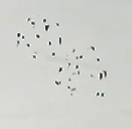
\includegraphics[width=0.2\textwidth]{./pic/u04-03-fig-01.png}
\caption{\label{fig:orgd55ec56}Geometric view of Gaussians}
\end{figure}

So in this case, you can still say, we have one Gaussian. This would be the
centroid of this Gaussian with a very high variance.

But we clearly see looking at this example that we actually have two clusters,
not a single cluster. Or if I may draw four, five, or six, you know, the more we
draw we can always say something like really one big Gaussian.

But if we can do much more refined modeling if our generative model can actually
explicitly allow us to talk about the fact that we have several different
clusters. And that's exactly where we're introducing these mixture models.

When we are talking about mixture models, we would assume that we have several
mixture components, each one of them will be a Gaussian:

\begin{equation}
\label{eq:org5ae6573}
K, \mathcal{N}(x, \mu^{(j)}, \sigma_{j}^{2}); j=1 \ldots K 
\end{equation}

So we will have, let's say, \(K\), the size of our mixture model. And then we
would assume that each Gaussian would be represented by its own private \(mu\)
and \(\sigma^2\).

So now, in this particular case, we will have two components, where \(j\) would
go from \(1\) to \(2\) and each one of them would have its own mean and its own
variance.

So now, it should be already reminding you of our conversation about clustering,
because in the case of clustering, you had several clusters, and we described
each class to maybe be representative of that cluster. But here, we have the
next level of refinement. First of all, we are not only reporting the mean of
the cluster, we are actually looking at the variance. How spread is the cluster?
We would also introduce another piece that we want to capture here is how big is
this cluster? How likely is it this cluster takes more and more point? That's
why in addition to having \textbf{MIXTURE COMPONENTS}, we are also going to have
\textbf{MIXTURE WEIGHTS}.

And what mixture weights means is that now each one of these guys would come
with its own likelihood:

\begin{equation}
\label{eq:org3bd0a80}
\prob_1 \ldots \prob_K, \sum_{j=1}^{K} \prob_j = 1
\end{equation}

And this will be a multinomial. The sum of these probabilities would go to 1. So
this is a multinomial.

And we can think about the process of generating a point with this mixture model
as a 2-step process. The first step, you will kind of throw your dice and decide
which one of mixture component is used to generate our point.

So what we are going to do, we're going to first draw from our multinomial, when
we are selecting a particular cluster:

\begin{equation}
\label{eq:org790389a}
j \sim \text{multinomial} | (\prob_1 \ldots \prob_K)
\end{equation}

Then after I selected the cluster, it means that I selected already its \(\mu\)
of the cluster and \(\sigma^2\) of that cluster:

\begin{equation}
\label{eq:orgcbe378d}
x \sim \prob(x|\mu^{(j)}, \sigma_{j}^{2})
\end{equation}

So again, the process is imagine to yourself, you first have a dice. You throw
the dice. You find yourself a Gaussian and then you draw it from the Gaussian
according to its own parameters. So this is a generation step.

And another important distinction between this model and what we got when we
were doing k-means clustering, or any clustering, this is actually a soft
clustering model, because for every point that we have here, let's say we have
some \(\mu^{(1)}\) and \(\sigma_{1}^{2}\) here and \(\mu^{(2)}\) and
\(\sigma_{2}^{2}\) here, every single point here can be either generated by
\(\text{gaussian}_1\) or by \(\text{gaussian}_2\) just with different
probabilities.

So here, we have a much more refined way to talk about our distribution, because
every point kind of belongs to different components, just with different
likelihoods.

So this is our mixture model. So let's just think what kind of parameters we
have:

\begin{equation}
\label{eq:org534a41e}
\theta; \prob_1 \ldots \prob_K, \mu^{(1)} \ldots \mu^{(K)}, \sigma_{1}^{2} \ldots \sigma_{K}^{2}
\end{equation}

So again, our parameter \(\theta\), like we define above, the parameter set
would contain all the mixture weights, again represented by this polynomial,
then they're going to have \(\mu\) for each one of the components and then,
we're going to have \(\sigma^2\) for each one of these Gaussians.
\end{document}